\documentclass[11pt]{article}
\usepackage[a4paper,margin=1in]{geometry}
\usepackage{amsmath, amssymb}
\usepackage[dvips]{graphics}
\usepackage{hyperref}
\usepackage[margin=1in]{geometry}
\usepackage{amstext}
\usepackage{amsmath}
\usepackage{booktabs}
\usepackage{adjustbox}
\usepackage{array}



\usepackage{float}
\usepackage{caption2}
\setcaptionmargin{0.5in}
\usepackage{epsfig}
%\usepackage{psfrag}
\usepackage{color}
\graphicspath{{fig/}}
%\textwidth=6.531496in \textheight=9.031496in
%\usepackage{pslatex}
\usepackage{wrapfig}
\usepackage{setspace}
\usepackage{multirow}

\usepackage{fancyhdr}
\pagestyle{fancy}

\usepackage{algorithm2e}
\usepackage{algorithmic}

%\usepackage[noend]{algpseudocode}
%\usepackage{algorithm}
\usepackage{xcolor}



\title{Home Exam MVE441}
\author{Arvid Kolstad}
\date{\today}
\begin{document}
\maketitle
\section{Question 1(a)}


The dataset used was B11, containing 7680 training points with 820 input features across 7 classes. Label distribution is shown in table \ref{tab:classbalance_normal}. Input values range from $-12.725$ to $14.072$, with a mean of $0.419$ and standard deviation of $3.328$.

For dimensionality reduction, PCA was first applied but showed no clear elbow. Instead a $\frac{1}{x}$-shaped variance curve, indicating high variance across all features without class-specific information. Since PCA is unsupervised, F-statistics (sklearn.feature\_selection.r\_regression) were used instead to identify class-correlated features. A clear elbow appeared at around 20 features (figure \ref{fig:ftest_data}), which were adopted as the primary features for the remainder of the project. Since the F-test is linear, mutual information (\texttt{sklearn.feature\_selection.mutual\_info\_regression}) was also applied to catch any nonlinear correlations, but it identified the same features. All selected features had p-values well below $0.05$. To prevent adding features with 1 to 1 correlation, a correlation matrix were created (table \ref{table:correlation matrix}), were it's clear that no featuers have a correlation of 1 between each other.

Three models were selected: Logistic Regression (PyTorch), kNN (sklearn), and Regularized Discriminant Analysis (NumPy). Logistic Regression provides a strictly linear decision boundary, RDA models each class with Gaussian distributions and adapts well to varying data sizes, and kNN makes no distributional assumptions while capturing highly complex boundarie, three contrasting approaches.

Model evaluation followed the same nested cross-validation pipeline as project 3: the inner kCV ran 3 times, the outer 5 times, repeated 10 times to assess variance, were the kCV always used stratification to create folds. Hyperparameters were tuned using Bayesian optimisation (scikit-optimize), with 20 evaluations per outer fold were the 10 first had a focus on exploration and 10 last had a focus on performance. Models were evaluated on accuracy and macro F1-score, where each class contributes equally regardless of its size. This was done to have a score that showed if a model was down-prioritizing minority classes. Model comparison used Bayesian analysis (Baycomp), with the ROPE determined by running the pipeline on randomly labelled data and set such that the mean probability of equivalent performance exceeded $95\%$, and this was set to $4\%$.

The results of the pipeline can be found in figure \ref{fig:performance_problem1}. We can see that the performance is around high 80\% to low 90\% for the 200 sample size, and goes rapidly up to around 95\% for 1000 sample sizes and from there slowly creeps upward from this. We also see that the variance of the scores are slowly reduces with the increase of sample size which is expected. Both scores is quite similar with the exception that f1-score is a bit lower for Logistic Regression and kNN in the beginning. This makes sense if we look at the class accuracy in figure \ref{fig:class_accuracy}. We can see that for 200 samples both escpecially kNN had a hard time classifying class 3 which makes sense as this is by far the smallest class in the dataset. If we look at the variance of the accuracy of class 3 we can also see that his is the largest for all the models when the sample size is small, which is expected. Looking at figure \ref{fig:bayesian_compare_problem1} we can see that in the beginning the Regularized Discriminant Analysis is the clear winner but around 1000 samples they all score within the rope. This is expected because of RDAs ability to adapt it self after small sample sizes.
\newpage

\subsection{Conclusions}
\begin{itemize}
	\item The dataset is fairly balanced were most of the classes has appears around 15\% with the exception of class number 3 that only has 6.2\% of the labels.

	\item The index of features that were relevant for the classification task where the following: 7, 37, 100,141, 158, 179, 210, 228, 276, 308, 410, 427, 519, 550, 558, 597, 752, 762, 796, 809. Checking the correlation matrix for these matrices confirmed that none of these features were exactly the same.
	\item The models does a good job of classifying the dataset with accuracy and F1 scores around 90\% for most of the sample sizes. KNN and Logistic Regression does a bit worse on the smallest sample sizes compared to RDA but this expected because of RDAs ability to adapt with LDA and Native Bayes which is known to performe great on smaller sample sizes.
	\item For smaller sample sizes the accuracy and performance for class 3 is noticable worse than for other classes which is expected. For larger sample sizes the hardest class instead becomes class 7 for all the models. This could be because of the class distribution in features.

\end{itemize}

\newpage
\begin{table}[H]
	\begin{center}
		\begin{tabular}{|c|c|c|c|c|c|c|c|}
			\hline
			\textbf{Class} & \textbf{1} & \textbf{2} & \textbf{3} & \multicolumn{1}{c|}{4} & \multicolumn{1}{c|}{\textbf{5}} & \multicolumn{1}{c|}{\textbf{6}} & \multicolumn{1}{c|}{\textbf{7}} \\ \hline
			Fraction       & $15.6\%$   & $15.6\%$   & $6.2\%$    & $15.8\%$               & $14.1\%$                        & $15.6\%$                        & $17.2\%$                        \\ \hline
		\end{tabular}
		\caption{This table shows the balance over the dataset. The smallest class of the dataset is class 3 and the largest class is 7.}
		\label{tab:classbalance_normal}
	\end{center}
\end{table}

\begin{figure}[H]
	\begin{center}
		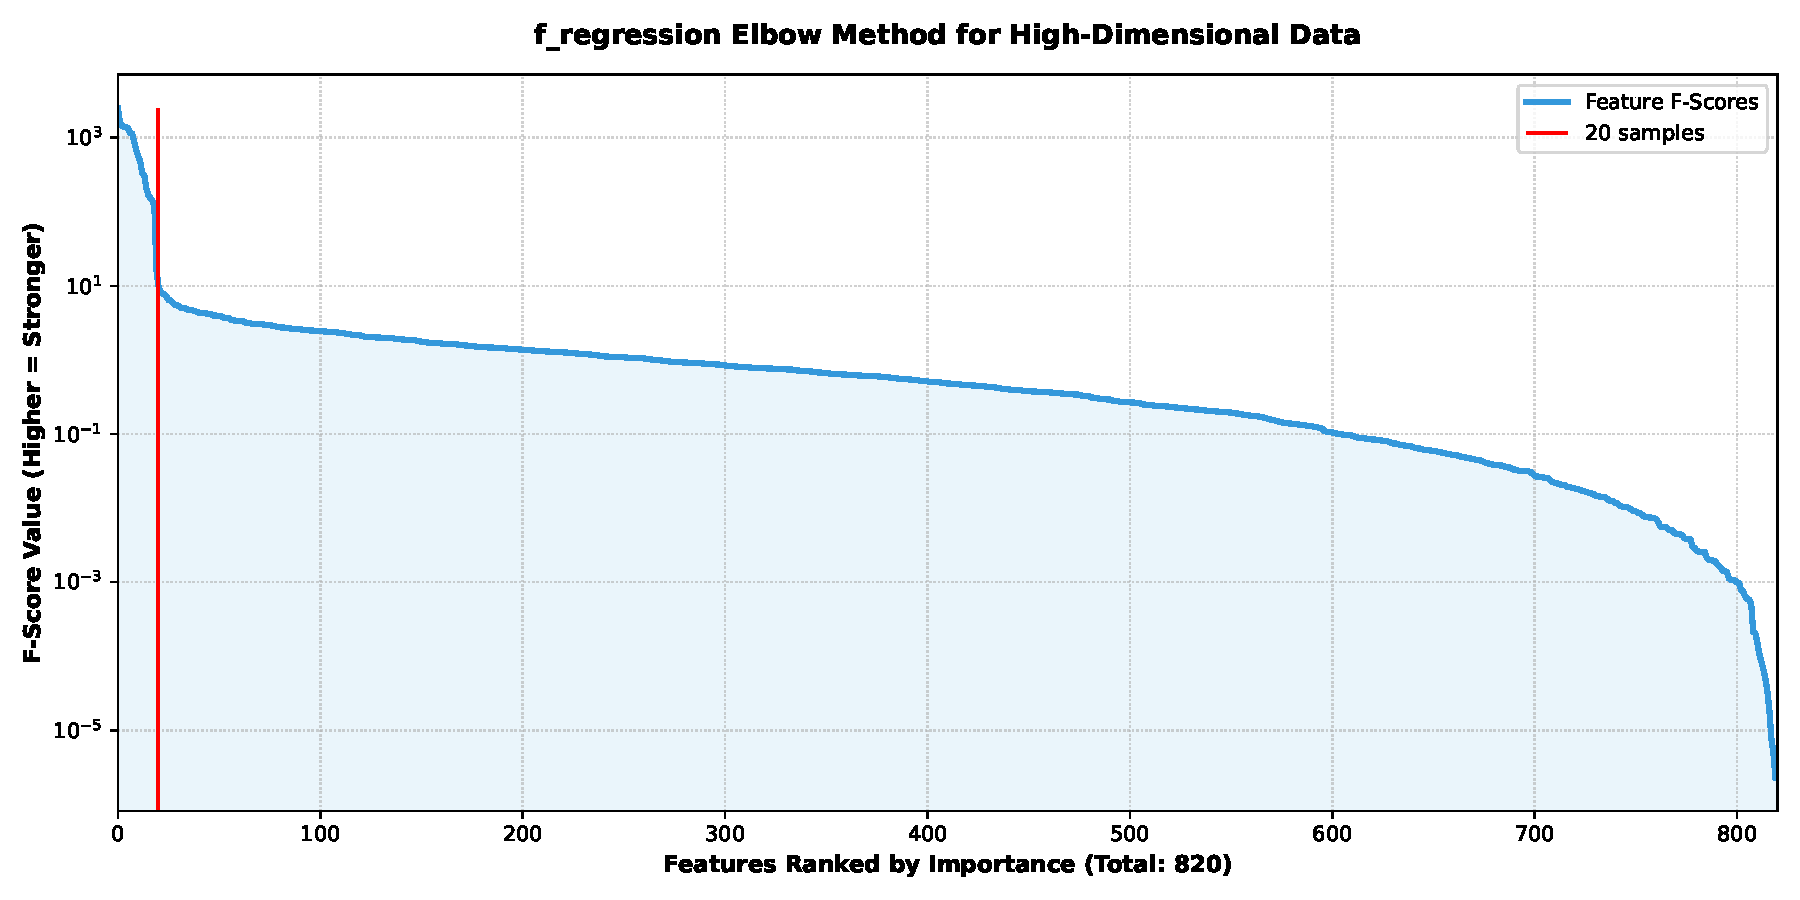
\includegraphics[width=0.99\textwidth]{../figures/vis_data/show_elbow.pdf}
	\end{center}
	\caption{In this figure we can see the F-Score plotted from highest to lowest. We can see a clear elbow after 20 features, and therefore these are the features we will use in the rest of the project.}\label{fig:ftest_data}
\end{figure}

\begin{table}[ht]
	\centering
	\begin{adjustbox}{max width=\textwidth}
		\begin{tabular}{r|rrrrrrrrrrrrrrrrrrrr}
			\toprule
			             & \textbf{7} & \textbf{37} & \textbf{100} & \textbf{141} & \textbf{158} & \textbf{179} & \textbf{210} & \textbf{228} & \textbf{276} & \textbf{308} & \textbf{410} & \textbf{427} & \textbf{519} & \textbf{550} & \textbf{558} & \textbf{597} & \textbf{752} & \textbf{762} & \textbf{796} & \textbf{809} \\
			\midrule
			\textbf{7}   & 1.00       & 0.18        & 0.49         & 0.33         & -0.40        & 0.59         & -0.39        & 0.24         & -0.27        & 0.51         & -0.19        & -0.06        & -0.08        & 0.33         & -0.33        & -0.35        & 0.18         & 0.69         & -0.21        & -0.05        \\
			\textbf{37}  & 0.18       & 1.00        & 0.06         & -0.12        & 0.41         & 0.19         & 0.23         & 0.32         & 0.54         & 0.37         & -0.50        & -0.35        & -0.30        & -0.19        & 0.48         & -0.18        & -0.27        & 0.18         & -0.08        & -0.21        \\
			\textbf{100} & 0.49       & 0.06        & 1.00         & 0.16         & -0.37        & 0.51         & -0.52        & 0.24         & -0.15        & 0.54         & -0.39        & -0.10        & -0.16        & 0.51         & -0.30        & -0.47        & -0.05        & 0.60         & -0.18        & -0.19        \\
			\textbf{141} & 0.33       & -0.12       & 0.16         & 1.00         & -0.39        & 0.41         & -0.24        & -0.01        & -0.31        & 0.31         & 0.19         & 0.23         & 0.24         & 0.31         & -0.28        & -0.13        & 0.28         & 0.46         & 0.24         & 0.03         \\
			\textbf{158} & -0.40      & 0.41        & -0.37        & -0.39        & 1.00         & -0.30        & 0.50         & 0.07         & 0.72         & -0.18        & -0.28        & -0.31        & -0.15        & -0.37        & 0.69         & 0.17         & -0.46        & -0.45        & 0.17         & -0.22        \\
			\textbf{179} & 0.59       & 0.19        & 0.51         & 0.41         & -0.30        & 1.00         & -0.40        & 0.23         & -0.07        & 0.56         & -0.37        & -0.14        & -0.04        & 0.31         & -0.21        & -0.50        & 0.10         & 0.69         & -0.03        & -0.20        \\
			\textbf{210} & -0.39      & 0.23        & -0.52        & -0.24        & 0.50         & -0.40        & 1.00         & 0.02         & 0.36         & -0.20        & 0.16         & 0.07         & -0.06        & -0.40        & 0.51         & 0.41         & -0.22        & -0.45        & 0.01         & 0.13         \\
			\textbf{228} & 0.24       & 0.32        & 0.24         & -0.01        & 0.07         & 0.23         & 0.02         & 1.00         & 0.23         & 0.47         & -0.34        & -0.22        & -0.24        & -0.06        & 0.14         & -0.17        & -0.18        & 0.24         & -0.14        & -0.03        \\
			\textbf{276} & -0.27      & 0.54        & -0.15        & -0.31        & 0.72         & -0.07        & 0.36         & 0.23         & 1.00         & 0.12         & -0.53        & -0.38        & -0.27        & -0.36        & 0.69         & -0.05        & -0.51        & -0.21        & 0.13         & -0.31        \\
			\textbf{308} & 0.51       & 0.37        & 0.54         & 0.31         & -0.18        & 0.56         & -0.20        & 0.47         & 0.12         & 1.00         & -0.45        & -0.16        & -0.26        & 0.19         & -0.05        & -0.44        & -0.10        & 0.67         & -0.18        & -0.11        \\
			\textbf{410} & -0.19      & -0.50       & -0.39        & 0.19         & -0.28        & -0.37        & 0.16         & -0.34        & -0.53        & -0.45        & 1.00         & 0.52         & 0.35         & -0.01        & -0.25        & 0.52         & 0.37         & -0.32        & 0.07         & 0.46         \\
			\textbf{427} & -0.06      & -0.35       & -0.10        & 0.23         & -0.31        & -0.14        & 0.07         & -0.22        & -0.38        & -0.16        & 0.52         & 1.00         & 0.29         & 0.18         & -0.27        & 0.29         & 0.30         & -0.10        & 0.17         & 0.38         \\
			\textbf{519} & -0.08      & -0.30       & -0.16        & 0.24         & -0.15        & -0.04        & -0.06        & -0.24        & -0.27        & -0.26        & 0.35         & 0.29         & 1.00         & 0.19         & -0.14        & 0.16         & 0.22         & -0.09        & 0.26         & 0.06         \\
			\textbf{550} & 0.33       & -0.19       & 0.51         & 0.31         & -0.37        & 0.31         & -0.40        & -0.06        & -0.36        & 0.19         & -0.01        & 0.18         & 0.19         & 1.00         & -0.38        & -0.23        & 0.14         & 0.37         & 0.08         & -0.16        \\
			\textbf{558} & -0.33      & 0.48        & -0.30        & -0.28        & 0.69         & -0.21        & 0.51         & 0.14         & 0.69         & -0.05        & -0.25        & -0.27        & -0.14        & -0.38        & 1.00         & 0.15         & -0.41        & -0.34        & 0.11         & -0.16        \\
			\textbf{597} & -0.35      & -0.18       & -0.47        & -0.13        & 0.17         & -0.50        & 0.41         & -0.17        & -0.05        & -0.44        & 0.52         & 0.29         & 0.16         & -0.23        & 0.15         & 1.00         & -0.04        & -0.54        & 0.04         & 0.34         \\
			\textbf{752} & 0.18       & -0.27       & -0.05        & 0.28         & -0.46        & 0.10         & -0.22        & -0.18        & -0.51        & -0.10        & 0.37         & 0.30         & 0.22         & 0.14         & -0.41        & -0.04        & 1.00         & 0.19         & 0.02         & 0.23         \\
			\textbf{762} & 0.69       & 0.18        & 0.60         & 0.46         & -0.45        & 0.69         & -0.45        & 0.24         & -0.21        & 0.67         & -0.32        & -0.10        & -0.09        & 0.37         & -0.34        & -0.54        & 0.19         & 1.00         & -0.22        & -0.14        \\
			\textbf{796} & -0.21      & -0.08       & -0.18        & 0.24         & 0.17         & -0.03        & 0.01         & -0.14        & 0.13         & -0.18        & 0.07         & 0.17         & 0.26         & 0.08         & 0.11         & 0.04         & 0.02         & -0.22        & 1.00         & -0.10        \\
			\textbf{809} & -0.05      & -0.21       & -0.19        & 0.03         & -0.22        & -0.20        & 0.13         & -0.03        & -0.31        & -0.11        & 0.46         & 0.38         & 0.06         & -0.16        & -0.16        & 0.34         & 0.23         & -0.14        & -0.10        & 1.00         \\
			\bottomrule
		\end{tabular}

	\end{adjustbox}
	\caption{A table over the correlation matrix for the 20 features that was picked out from the F-Test. No other correlation is close to 1.00 in this table which shows that all of these features are needed for the classificationt task.\label{table:correlation matrix}}


\end{table}

\begin{figure}[H]
	\begin{center}
		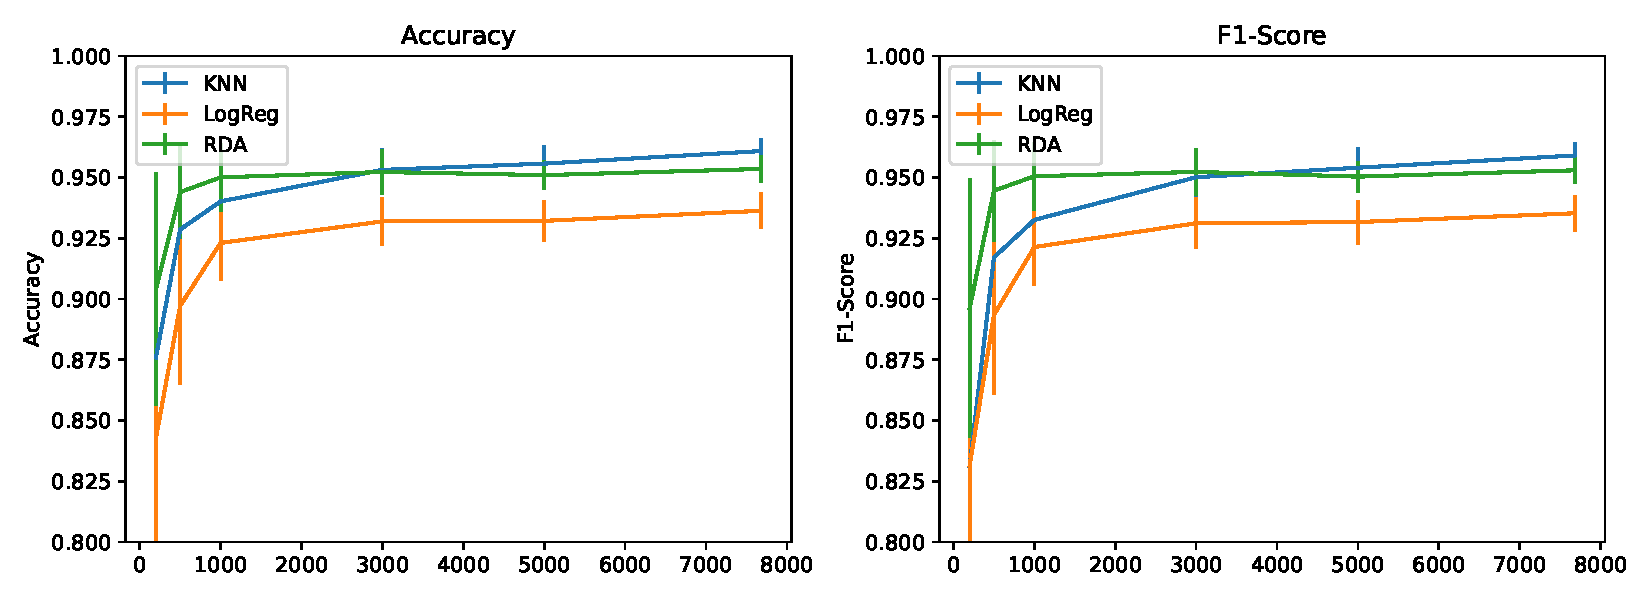
\includegraphics[width=0.99\textwidth]{../figures/problem1/performance.pdf}
	\end{center}
	\caption{In this figure presents the performance for the diffetent models after running the pipeline over different sample sizes. The left plot displays the accuracy score and the right plot shos the F1-score. We can see that Logistic Regression is performing the worst, and the KNN and RDA is almost similar in their performance over different sample sizes.}\label{fig:performance_problem1}
\end{figure}
\begin{figure}[H]
	\begin{center}
		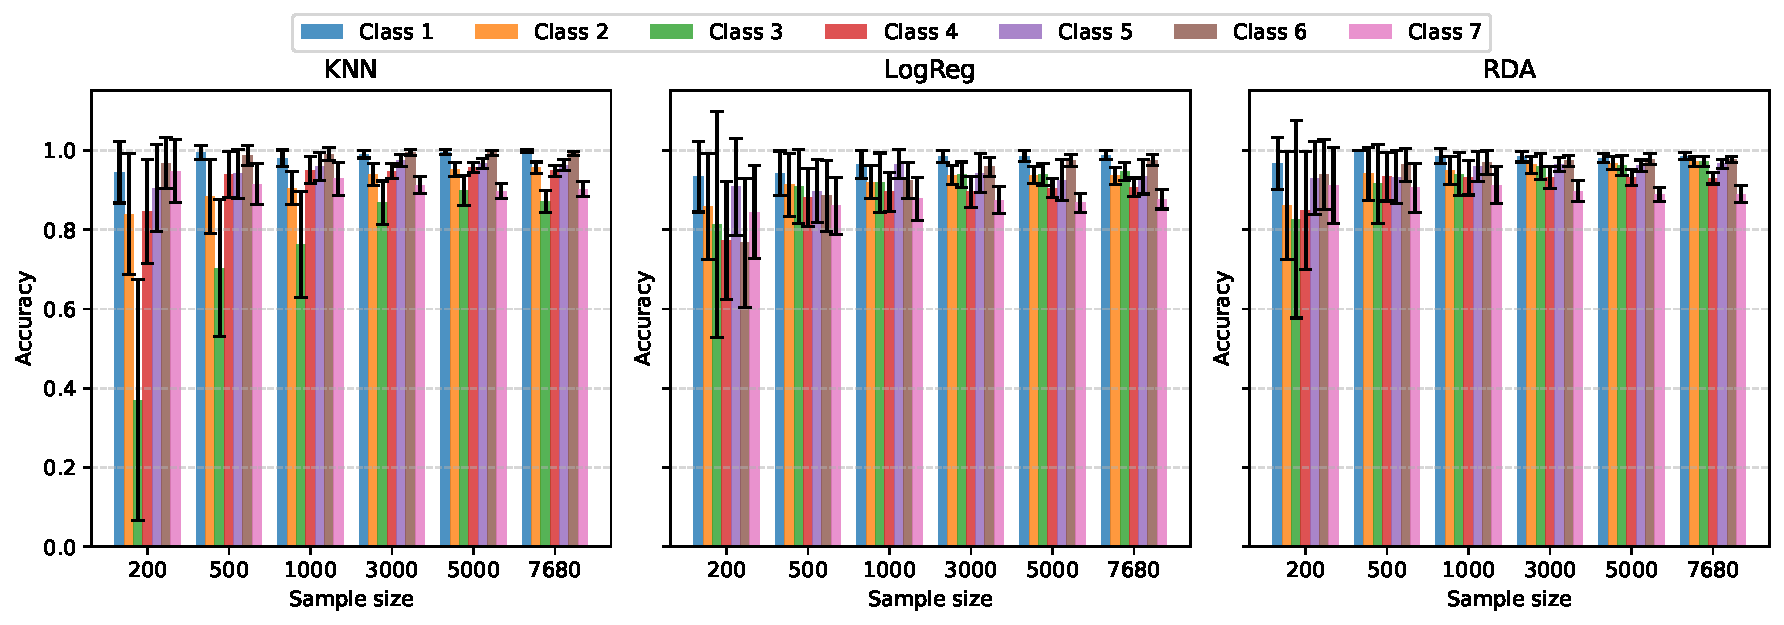
\includegraphics[width=0.99\textwidth]{../figures/problem1/class_accuracy.pdf}
	\end{center}
	\caption{In this figure we can see each models accuuracy per class. While performing the worst for smaller sample sizes, escpecially for class 3, the accuracy is quite similar for higher sample sizes. }\label{fig:class_accuracy}
\end{figure}
\begin{figure}[H]
	\begin{center}
		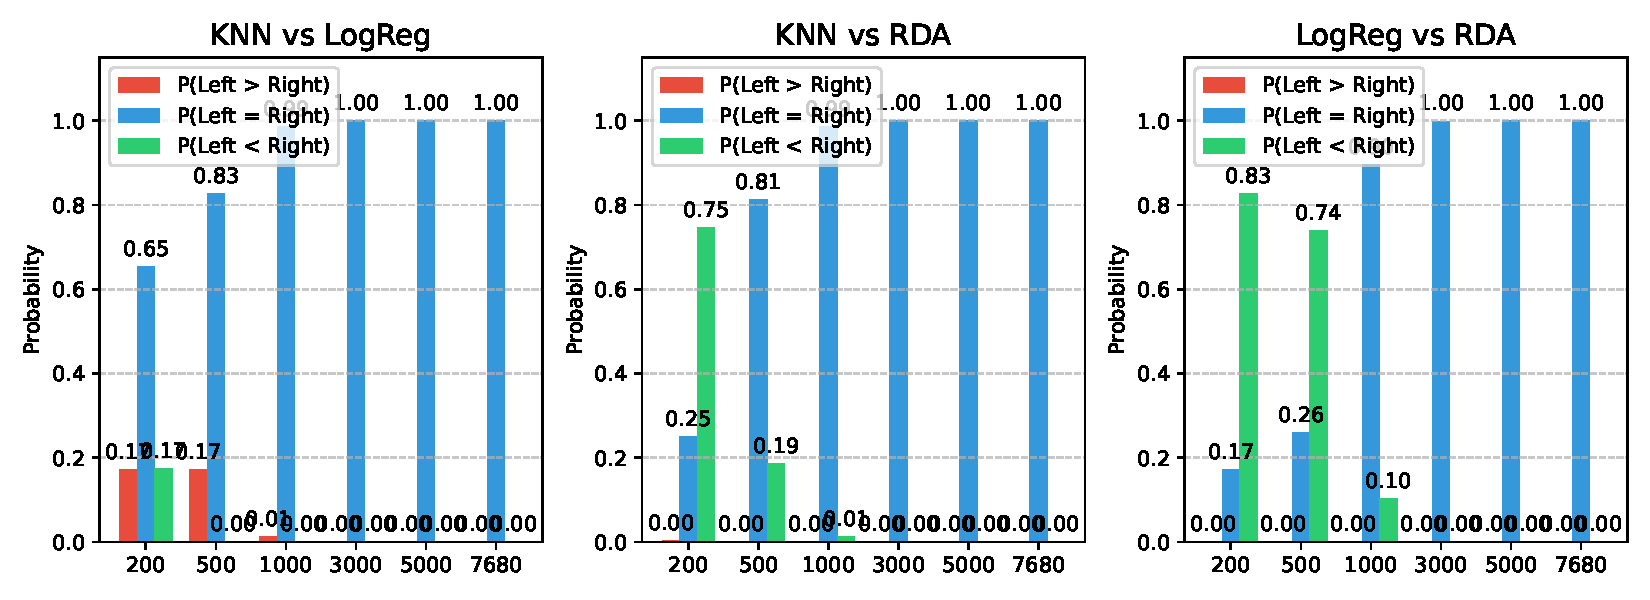
\includegraphics[width=0.99\textwidth]{../figures/problem1/bayes_comp.pdf}
	\end{center}
	\caption{In this picture we can see the bayesian comparisons between the models, were the performance score used is F1-score. While RDA is performing the best in the beginning, the KNN and LogReg is fast to catch up around 1000 in sample size. The rope that was used for the comparison were $4\%$.}\label{fig:bayesian_compare_problem1}
\end{figure}








\newpage
\section{Question 1(b)}
To address this question, a controlled disruption was introduced to the dataset to intentionally degrade model performance. Specifically, a variable number of randomly selected features from the original 820 features were injected as noise to study the models' robustness. The evaluation pipeline described in Question 1(a) was utilized to measure performance. For each iteration of the pipeline, a new set of random features was sampled to ensure an unbiased and comprehensive assessment of the models' behavior. All 7,600 samples were used across all runs to obtain the most accurate measure of performance degradation. To evaluate the impact, we analyze the performance metrics across all models and perform a Bayesian analysis to compare the F1-scores. The Region of Practical Equivalence (ROPE) for this analysis was defined based on the standard deviation of the original baseline model.

Figure~\ref{fig:performance} illustrates the performance of the models as a function of the increasing number of noisy features used during training and classification. RDA demonstrates notable robustness against this noise; in fact, for the first few added features, the model's performance increases in terms of both accuracy and F1-score. This behavior is expected given RDA's capacity to adapt to noisy dimensions by tuning its hyperparameters toward LDA or Naive Bayes. This mechanism acts similarly to an ridge regularizer on these parameters, allowing the model to potentially leverage these features rather than allowing them to obscure the class signal. This phenomenon is clearly visible in Figure~\ref{fig: Comparison_degraded}, where the model initially leverages the injected features to its advantage.

As anticipated, the kNN model exhibited the sharpest decline in performance. As shown in Figure~\ref{fig:performance}, the mean values for both accuracy and F1-score drop after the introduction of just a single noisy dimension, and performance continues to monotonically degrade as more dimensions are added. Furthermore, the Bayesian comparison in Figure~\ref{fig: Comparison_degraded} reveals that the baseline model achieves a higher probability of superiority after only 5 additional dimensions. This confirms that kNN is highly sensitive to noise, likely because the irrelevant dimensions distort the distance metrics, thereby disrupting the local neighborhood structure and degrading classification accuracy.

Logistic Regression also failed to benefit from the additional dimensions. Figure~\ref{fig:performance} shows that the model's accuracy and F1-score begin to decline after approximately 3 to 5 extra features are introduced. While it proves more resilient than kNN, its performance falls significantly short of RDA. This outcome was somewhat surprising, as Logistic Regression was expected to maintain stability due to its Ridge regularization; however, this penalty proved insufficient to counteract the noise. Figure~\ref{fig: Comparison_degraded} confirms that the model's performance becomes significantly worse after the introduction of roughly 15 to 20 extra features.

\newpage
\subsection{Conclusions}
\begin{itemize}
	\item The introduction of random features was sufficient to degrade the performance of several models.
	\item RDA demonstrated the highest robustness, initially showing an improvement in accuracy before the trend dissipated and performance reverted toward its baseline as more features were added.
	\item kNN suffered the most severe performance degradation, which aligns with expectations given the model's inherent sensitivity to noise.
	\item The extent to which Logistic Regression was affected was unexpected. While Ridge regularization was anticipated to mitigate the impact of noise, it proved insufficient, suggesting that Lasso regularization might have been more effective at feature selection in this scenario.
\end{itemize}
\begin{figure}
	\begin{center}
		
\includegraphics[width=0.95\textwidth]{../figures/problem2/performance.pdf}
	\end{center}
	\caption{This figure shows the performance over extra features that was added to the inputs. You can see that the RDA model performance was not noticable compared to the other models. The kNN had the worst performance drop out of the models which was expectend because of the models sensitivity to noise.}\label{fig:performance}
\end{figure}

\begin{figure}[H]
	\begin{center}
		
\includegraphics[width=0.95\textwidth]{../figures/problem2/bayes_comp.pdf}
	\end{center}
	\caption{This figure shows the comparison with baysian analysis between the models original performance and the performance with added features. We can see that for the kNN and the LogReg the original model is performing better after a couple of added features, but RDA keeps it performance steady and even improves in the beginning.}\label{fig: Comparison_degraded}
\end{figure}
\newpage
\section{Question 1(c)}
The question here is to conclude if the dataset that is being used in this project contains any mislabels. To do this, a procentage of how sure every model was on its prediction was obtained. From Logistic Regression the softmax from each of it's 7 outputs was taken, for kNN it uses the number of neighbors in that class divided by the total number of neighbors and RDA calculates its confidence by measuring how close a data point is to each class center, adjusted for the regularized shape of the cluster, combining that distance with the overall commonness of the class, and using a softmax function to turn those scores into a final percentage split.

To create a method that can find mislabels in the data, a threshold of 5\% was set. If a model clasifies a data point, which does not agree with the data points label, and the probability of the model classifying this as the actuall label is lower than the threshold, then it will mark that point. If all the models mark the data point, then the the label will get classified as a mislabeled point. The false positive rate of this is calculated as following given that the models prediction is correct and that the models are independent of each other:
\begin{equation}
	P(\text{model mislabeling a point}) = (1 - (1-threshold)^{10})^3 \approx 40.13\%
	\label{eq:}
\end{equation}
which makes all three models have a false positive at the same time as $(40.13\%)^3 = 6.5\%  $  which makes it of course possible but not a big part of the data set anyway.

The result of this study can be found in table \ref{tab:mislabels_results}, were 75 mislabels were found and 195 of my 200 labels were correctly identified as wrong. This gives a false negative of about 2.5\% which is great. In table \ref{class_misslabels} you can see the differnt types of mislabelings. The most common mislabeling is the class 4 mislabeled as a 4, and the other mislabels is just one or two.


\newpage

\subsection{Conclusions}
\begin{itemize}
	\item The model that was created was abel, given that the prediction from the model is correct, with a calculated false positive of 6.5\% and a experimental value of false negative of 2.5\%.
\end{itemize}
\newpage

\begin{table}[H]
	\centering

	\begin{tabular}{|c|c|}
		\hline
		\textbf{\begin{tabular}[c]{@{}c@{}}Mislabels\\ Original\end{tabular}} & \textbf{\begin{tabular}[c]{@{}c@{}}Mislabels\\ Faked\end{tabular}} \\ \hline
		75                                                                    & 195/200                                                            \\ \hline
	\end{tabular}
	\caption{Table over the mislabels found from the original data and the mislabels that the models caught that was introduced by me.}
	\label{tab:mislabels_results}
\end{table}
\begin{table}[H]
	\centering

	\newpage
	\begin{tabular}{llcl}
		\toprule
		\textbf{Labeled Class}   & \textbf{Probable Class} & \textbf{Number of times}   \\
		\midrule
		6                        & 4                       & 57                         \\
		2                        & 3                       & 4                          \\
		4                        & 2                       & 3                          \\
		4                        & 6                       & 2                          \\
		3                        & 2                       & 2                          \\
		1                        & 3                       & 2                          \\
		2                        & 5                       & 2                          \\
		4                        & 0                       & 1                          \\
		3                        & 1                       & 1                          \\
		3                        & 5                       & 1                          \\
		\midrule
		\textbf{Total Mislabels} &                         & \textbf{75}              & \\
		\bottomrule
	\end{tabular}
	\caption{This table summarizes the mislabelings that the models found and what the models thougt was the correct class. It's clear that the class with the most mislabelings were class 6 with a total of 57 mislabeling.\label{class_misslabels}}
\end{table}
\section{Question 1(d)}
In this question the two best performing models prediction confidence were to be studied. This is firslty
\newpage
\subsection{Conclusions}
\newpage

\begin{table}[]
	\centering
	\begin{tabular}{|c|c|}
		\hline
		\textbf{AUC- mean} & \textbf{AUC - STD} \\ \hline
		0.539              & 0.065              \\ \hline
	\end{tabular}
	\caption{Table over the AUC score that was obtained after training a random forest to distinguish between the training set and test set. This shows that the model can't distinguish between these sets which means that we can trust out predictions.}
	\label{tab:rf-score}
\end{table}

\begin{figure}
	\begin{center}
		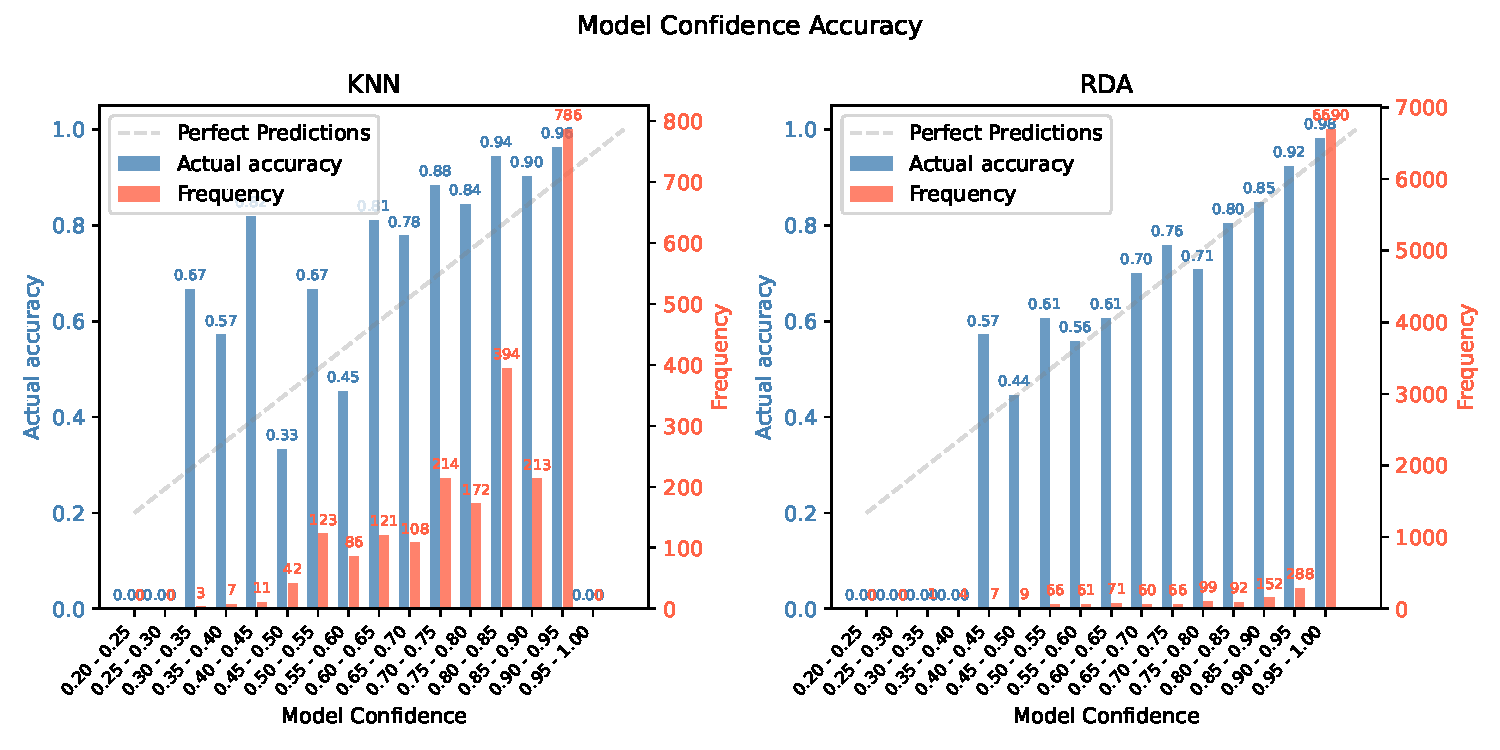
\includegraphics[width=0.95\textwidth]{../figures/problem3/model_conf_acc_7680.pdf}
	\end{center}
	\caption{}\label{fig:}
\end{figure}

\begin{figure}[H]
	\begin{center}
		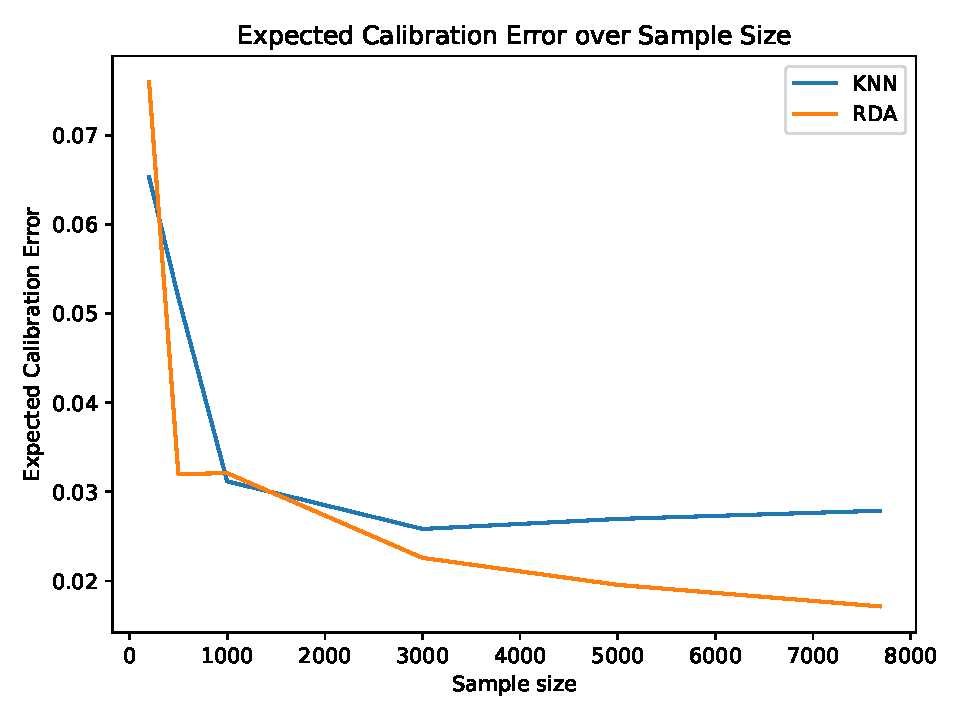
\includegraphics[width=0.95\textwidth]{../figures/problem3/conf_diff_sample_size.pdf}
	\end{center}
	\caption{}\label{fig:}
\end{figure}

\begin{figure}[H]
	\begin{center}
		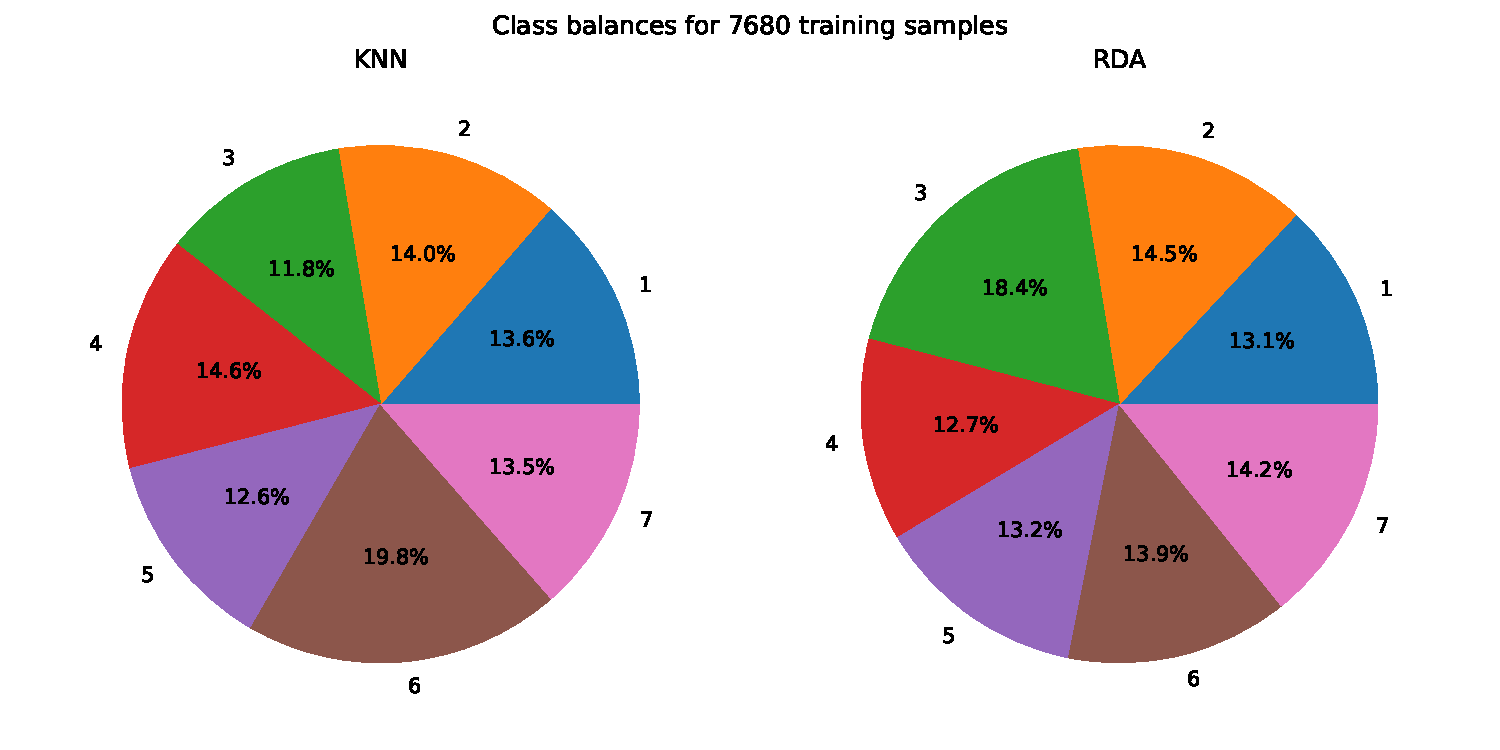
\includegraphics[width=0.95\textwidth]{../figures/problem3/class_balance_test.pdf}
	\end{center}
	\caption{}\label{fig:}
\end{figure}
\begin{figure}[H]
	\begin{center}
		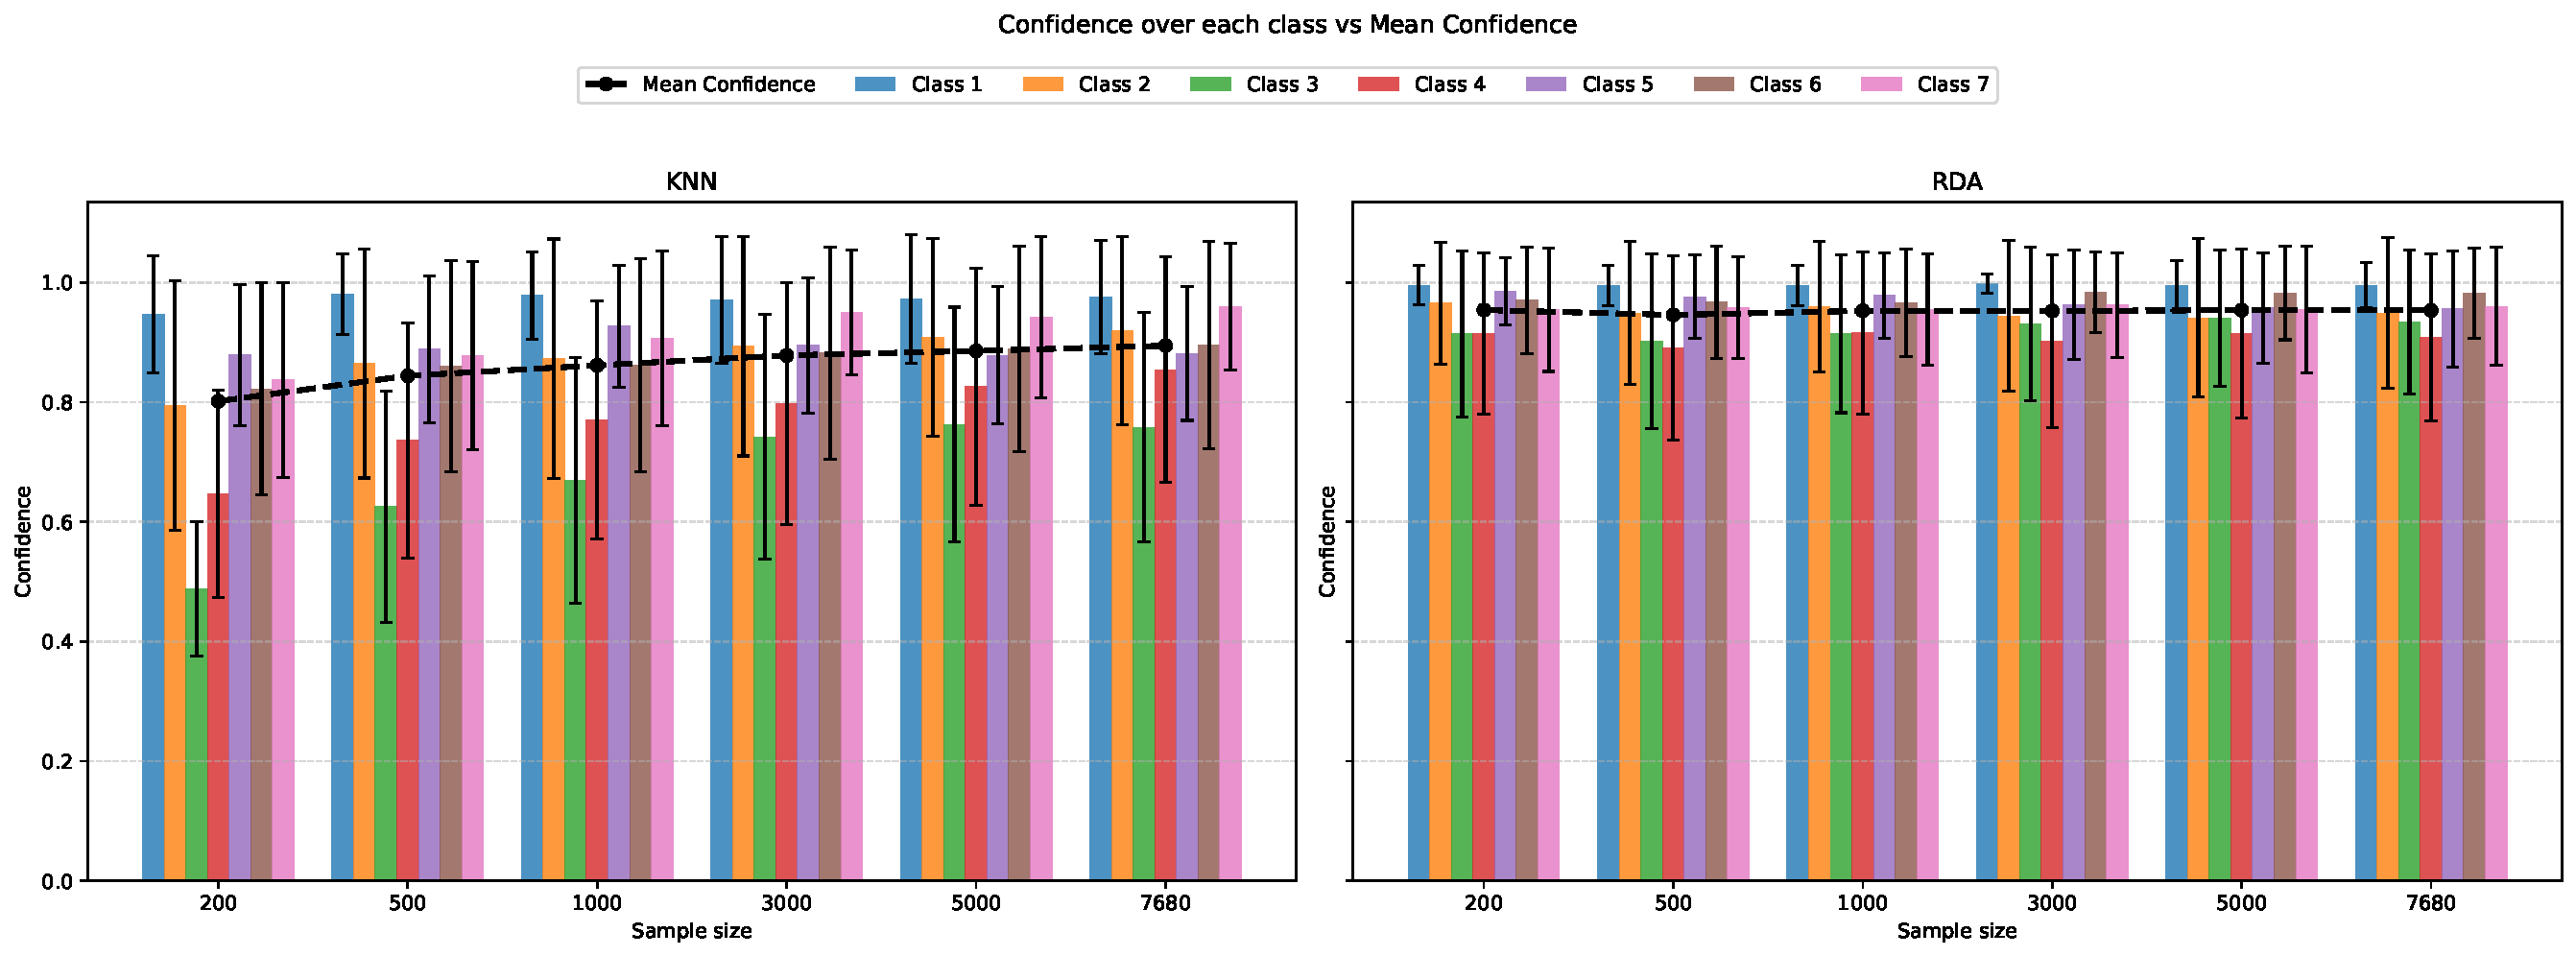
\includegraphics[width=0.95\textwidth]{../figures/problem3/test_confidence.pdf}
	\end{center}
	\caption{}\label{fig:}
\end{figure}





\end{document}

